\part{Graph and Network Theory}
	\chapter{Graph Theory}
		\section{Basic concepts}
		
		A \textbf{Graph} G consists of a finite set $V(G)$ on vertices, a finite set $E(G)$ on edgesand an \textbf{incident relation} than associates with any edge $e\in E(G)$ an unordered pair of vertices not necessarily distinct called \textbf{ends}.

		\begin{figure}[h!]
			\centering
			\begin{tikzpicture}[node distance = 2cm]
				\node (v_2) [circleNode] {$v_2$};
				\node (v_3) [circleNode, right of = v_2] {$v_3$};
				\node (v_1) [circleNode, below of = v_2] {$v_1$};
				\node (v_4) [circleNode, below of = v_3] {$v_4$};
				\node (v_5) [circleNode, right of = v_3] {$v_5$};
				\node (v_6) [circleNode, below of = v_5] {$v_6$};
				\draw [link] (v_2) -- node [left] {$e_2$} (v_1);
				\draw [link] (v_2) -- node [below] {$e_5$} (v_4);
				\draw [link] (v_1) to [out = 180, in = 270, looseness = 5] node [right] {$e_1$} (v_1);
				\draw [link] (v_2) to [out = 45, in = 135] node [above] {$e_3$} (v_3);
				\draw [link] (v_2) to [out = 315, in = 225] node [above] {$e_4$} (v_3);
				\draw [link] (v_3) -- node [right] {$e_6$} (v_1);
				\draw [link] (v_5) -- node [right] {$e_7$} (v_6);
			\end{tikzpicture}			
		\end{figure}

		It can be represented as
		\begin{align}
			V = V(G) = \{v_1, v_2, v_3, v_4, v_5, v_6\} \\
			E = E(G) = \{e_1, e_2, e_3, e_4, e_5, e_6, e_7\}\\
			e_1 = v_1v_2, e_2 = v_2v_4, ...
		\end{align}

		Serveral concepts: \\
		\indent - An edge with identical ends is called a \textbf{loop}\\
		\indent - Two edges having the same ends are said to be \textbf{parallel}\\
		\indent - A graph without loops or parallel edges is called \textbf{simple graph}\\
		\indent - two edges of a graph are \textbf{adjancent} if they have a common end\\
		\indent - two vertices are \textbf{adjancent} if they are jointed by an edge\\
		

	\section{Subgraph}

		Given two graphs \textbf{G} and \textbf{H}, \textbf{H} is a \textbf{subgraph} of \textbf{G} if $V(H)\subseteq V(G)$, $E(H)\subseteq E(G)$ and an edge has the smae ends in \textbf{H} as it does in \textbf{G}, if $E(H)\neq E(G)$ then \textbf{H} is a proper subgraph.

		A subgraph \textbf{H} on \textbf{G} is \textbf{spanning} if $V(H) = V(G)$

		For a subset $V^{'}\subseteq V(G)$ we define an \textbf{vertex-induced} subgraph $G[V^{'}]$ to be the subgraph with vertices $V^{'}$ and those edges of \textbf{G} having both ends in $V^{'}$

		The \textbf{edge-induced} subgraph $G[E^{'}]$ has edges $E^{'}$ and those vertices of \textbf{G} that are ends to edges in \textbf{$E^{'}$}

		If we combine node-indeced or edge-induced subgraphs $G(V^{'})$ and $G(V - V^{'})$, we cannot get the entire graph.

		Let $v\in V(G)$, then the \textbf{degree} of $v\in V(G)$ denote by $d_G(v)$ is defines to be the number of edges incident of $v$. Loops counted twice.

		\begin{theorem}
			For any graph \textbf{G=(V, E)}
			\begin{equation}
				\sum_{v\in V}d(v) = 2|E|
			\end{equation}			
		\end{theorem}

		\begin{proof}
			$\forall$ edge $e=\mu v$ with $\mu \neq v$, $e$ is  and counted once for $\mu$ and once for $v$, a total of two altogether. If $e=\mu \mu$, a loop, then it is counted twice for $\mu$			
		\end{proof}

		\begin{corollary}
			Every graph has an even number of odd degree vertices.
		\end{corollary}

		\begin{proof}
			\begin{equation}
				V = V_E\cup V_O \Rightarrow 
				\sum_{v\in V}d(v) = \sum_{v\in V_E} d(v) + \sum_{v\in V_O}d(v) = 2|E|
			\end {equation}			
		\end{proof}


	\chapter{Paths, Trees, and Cycles}
		\section{Walk}

			A \textbf{walk} in a graph \textbf{G} is a finite sequence $w=v_0e_1v_1e_2...e_kv_k$, where for each $e_i=v_{i-1}v_i$ the edge and its ends exists in \textbf{G}. We say that walk $v_0$ to $v_k$ on $(v_0, v_k)$-walk.
			\begin{equation}
				w = v_2e_4v_3e_4v_2e_5v_3
			\end{equation}
			is a walk, or $(v_2, v_3)$-walk\\
			The vertice $v_0$ and $v_k$ are called the \textbf{origin} and the \textbf{terminal} of the walk w.

			$v_1..v_{k-1}$ are called \textbf{interal} vertices

	 		The integer $k$ is the \textbf{length} of the walk. Length of $w$ equals to the number of edges.

	 		We can create a reverse walk $w^{-1}$ by reversing $w$.
	 		\begin{equation}
	 			w^{-1} = v_ke_kv_{k-1}e_{k-1}...e_2v_1
	 		\end{equation}
	 		(The reverse walk is guaranteed to exist because it is an undirected graph)

	 		Given two walks $w$ and $w'$ we can create a third walk denoted by $ww'$ by concating $w$ and $w'$. The new walk's origin is the same as terminal.

	 	\section{Path and Cycle}

	 		A \textbf{trail} is a walk with \textbf{NO} repeating edges. e.g., $v_3e_4v_2e_5v_3$

	 		A \textbf{path} is a trail with \textbf{NO} repeating vertices. e.g., $v_3e_4v_2$

	 		Paths $\subseteq$ Trails $\subseteq$ Walks

	 		A path is \textbf{closed} if it has possitive length and its origin and terminal are the same. e.g., $v_1e_2v_2e_4v_3e_3v_1$

	 		A closed trail where origin and internal vertices are distincted is called a \textbf{cycle} (The only time a vertice is repeated is the origin and terminal)

	 		A cycle is \textbf{even} if it has a even number of edges otherwise it is \textbf{odd}.

	 		Two vertices $u$ and $v$ in a graph are said to be \textbf{connected} if there is a path between $u$ and $v$.

	 		Clearly connectivity between vertices is an equvalance relation on $V(G)$, if $V_1, ... V_k$ are the corresponding equivalent classes then $G[V_1]...G[V_k]$ are \textbf{components} of G.\\
	 		e.g., In the example, $G[V_1]$ and $G[V_2]$  are two component of V where $V_1={v_1, v_2, v_3, v_4}$ and $V_2={v_5, v_6}$

	 		if graph has only one component, then we say the graph is connected. A graph is connected iff every pair of vertices in G are connected, i.e., there exists a path between every pair of vertices.

	 	\section{Tree and forest}

			A graph is called \textbf{acyclic} if it has no cycles

	 		A acyclic graph is called a \textbf{forest}

	 		A connected forest is called a \textbf{tree}

	 		A subgraph T of G is a \textbf{spanning tree} if it is spanning ($V(T)=V(G)$) and it is a tree.

	 		For example in the following graph\\
	 		\begin{figure}[!h]
				\centering
				\begin{tikzpicture}[node distance = 2cm]
					\node (v_2) [circleNode] {$v_2$};
					\node (v_3) [circleNode, right of = v_2] {$v_3$};
					\node (v_1) [circleNode, below of = v_2] {$v_1$};
					\node (v_4) [circleNode, below of = v_3] {$v_4$};
					\node (v_5) [circleNode, right of = v_3] {$v_5$};
					\draw [link] (v_1) -- (v_2);
					\draw [link] (v_2) -- (v_3);
					\draw [link] (v_1) -- (v_4);
					\draw [link] (v_2) -- (v_4);
					\draw [link] (v_3) -- (v_5);
					\draw [link] (v_4) -- (v_5);
					\draw [link] (v_1) -- (v_3);
				\end{tikzpicture}			
			\end{figure}\\
			This is a spanning tree\\
	 		\begin{figure}[!h]
				\centering
				\begin{tikzpicture}[node distance = 2cm]
					\node (v_2) [circleNode] {$v_2$};
					\node (v_3) [circleNode, right of = v_2] {$v_3$};
					\node (v_1) [circleNode, below of = v_2] {$v_1$};
					\node (v_4) [circleNode, below of = v_3] {$v_4$};
					\node (v_5) [circleNode, right of = v_3] {$v_5$};
					\draw [link] (v_2) -- (v_3);
					\draw [link] (v_1) -- (v_4);
					\draw [link] (v_2) -- (v_4);
					\draw [link] (v_3) -- (v_5);
				\end{tikzpicture}			
			\end{figure}\\

			Every connected graph has a spanning tree.

			\begin{proof}
				We are going to use a algorithm proof.				
			\end{proof}

			Here is the algorithm:\\
			\begin{itemize}
				\item INPUT: a connected graph G and an enumeration $e_1,...e_m$ of the edges of G
				\item OUTPUT: a spanning tree T of G
			\end{itemize}

			\begin{algorithmic}[!ht]
				\STATE Let T be the spanning subgraph of $G$ with $V(T)=V(G)$ and $E(T)=\emptyset$
				\STATE $i \gets 1$
				\WHILE {$i \le |E|$}
					\IF {$T + e_i$ is acyclic}
						\STATE $T \gets T + e_i$
						\STATE $i \gets i + 1$
					\ENDIF
				\ENDWHILE
			\end{algorithmic}

			This algorithm can be optimized, one idea is to make summation of edges in spanning subgraph less or equation to $|V| - 1$

			To prove algorithm we need to show the output is a spaning tree, which means three properties must hold:
			\begin{itemize}
				\item spanning (Step I)
				\item acyclic (We never add an edge that create a cycle)
				\item connected (Proof by contradiction)
			\end{itemize}
			So it is sufficient to show that the output will be connected.
			\begin{proof}
				(Proof by Contradiction) Supposet the output graph $T$ of the algorithm is NOT connected. Let $T_1$ be a component of $T$, let $x\in T_1$ and $y \notin T_1$. But $G$ is a connected graph (given from the beginning), so there must be a path in $G$ that connects $x$ and $y$. Let such a path in $G$ be $p=xe_1v_1e_2,..v_{k-1}e_ky$. Clearly, $p\notin T_1$. So there must be a first vertex in $P$ that not in $T_1$. So $e_i \notin E(T)$, the only way this can happen when applying the algorithm is if $T + e_i$ creates a cycle $C$, i.e., $e_i \in C$, so $C - e_i$ is a path connecting $v_{i-1}$ and $v_i$. So $c - e_i \in T$, so $v_{i-1}$ is connected to $v_i \in T$. Contradiction. 
			\end{proof}

		\section{Special Graphs}
			\begin{definition}
				A \textbf{complete} graph $K_n (n \ge 1)$ is a simple graph with $n$ vertices and with exactly one edge between each pair of distinct vertices.
			\end{definition}

			\begin{definition}
				A \textbf{cycle} graph $C_n (n \ge 3)$ consists of $n$ vertices $v_1, ... v_n$ and $n$ edges $\{v_1, v_2\}, \{v_2, v_3\}, ... \{v_{n-1}, v_n\}$
			\end{definition}

			\begin{definition}
				A \textbf{wheel} graph $W_n (n \ge 3)$ is a simple graph obtains by adding one vertex to the cycle graph $C_n$, and connecting this new vertex to all vertices of $C_n$ 
			\end{definition}

			\begin{definition}
				A simple graph is said to be \textbf{bipantite} if the vertiex set can be expressed as the union of two disjoint non-exmpty subsets $V_1$ and $V_2$ such that every edges has one end in $V_1$ and another end in $V_2$
			\end{definition}

			\begin{figure}[!h]
				\centering
				\begin{tikzpicture}[node distance = 2cm]
					\node (A) [circleNode] {A};
					\node (B) [circleNode, right of = A] {B};
					\node (C) [circleNode, below of = A] {C};
					\node (D) [circleNode, right of = C] {D};
					\node (E) [circleNode, below of = C] {E};
					\node (F) [circleNode, right of = E] {F};
					\draw [link] (A) -- (B);
					\draw [link] (A) -- (D);
					\draw [link] (C) -- (B);
					\draw [link] (C) -- (F);
					\draw [link] (E) -- (D);
					\draw [link] (E) -- (F);
					\draw [link] (A) -- (F);
				\end{tikzpicture}
			\end{figure}

			The \textbf{complete bipartite} graph $K_{mn}$ is the bipartite graph $V_1$ containing $m$ vertices and $V_2$ containing $n$ vertices such that each vertiex in $V_1$ is adjacent to every vertex in $V_2$

			For example $K_{33}$
			\begin{figure}[!h]
				\centering
				\begin{tikzpicture}[node distance = 2cm]
					\node (A) [circleNode] {A};
					\node (B) [circleNode, right of = A] {B};
					\node (C) [circleNode, below of = A] {C};
					\node (D) [circleNode, right of = C] {D};
					\node (E) [circleNode, below of = C] {E};
					\node (F) [circleNode, right of = E] {F};
					\draw [link] (A) -- (B);
					\draw [link] (A) -- (D);
					\draw [link] (A) -- (F);
					\draw [link] (C) -- (B);
					\draw [link] (C) -- (D);
					\draw [link] (C) -- (F);
					\draw [link] (E) -- (B);
					\draw [link] (E) -- (D);
					\draw [link] (E) -- (F);
				\end{tikzpicture}
			\end{figure}

		\section{Complexity}
			How do we measure the efficiency of an algorithm?

			We mostly measure on "worse case" scenarios.

			We want to know guarenteed perpormances for any algorithm working on any problem instance.

			Example: Add two $m \times n$ matrices $A$, $B$ to get matrix $C$
			\begin{algorithmic}[!h]
				\FOR {$i=1, 2, ..., m$}
					\FOR {$j=1, 2, ..., n$}
						\STATE $C_{ij} = A_{ij} + B_{ij}$
					\ENDFOR
				\ENDFOR
			\end{algorithmic}
			The "running time" of an algorithm is measured by the number of basic operational steps.

			For so called "basic" steps, it includes
			\begin{itemize}
				\item $+$, $-$, $\times$, $\div$
				\item assignments and storage of a variable
				\item comparisions
			\end{itemize}

			For the example above
			\begin{itemize}
				\item $c_1 m n$ for addition $C_{ij} = A_{ij} + B_{ij}$
				\item $c_2 m n$ for saving $C_{ij}$
				\item $c_3 m n$ for comparision and assignment for $i$ and $j$
			\end{itemize}
			$c_1, c_2, c_3$ does not matter, the number of steps are $m \times n$, we say the algorithm runs $O(mn)$ (big O notation, the worse case)

	\chapter{Shortest-Path Problem}

	\chapter{Minimum Spanning Tree Problem}

	\chapter{Maximum Flow Problem}

	\chapter{Minimum Cost Flow Problem}

	\chapter{Assignment and Matching Problem}

	\chapter{Graph Algorithms}

	\chapter{Polygon Triangulation}
		\section{Types of Polygons}
			\begin{definition}
				A \textbf{simple polygon} is a closed polygonal curve without self-intersection.
			\end{definition}
			\begin{figure}[h!]
				\centering
				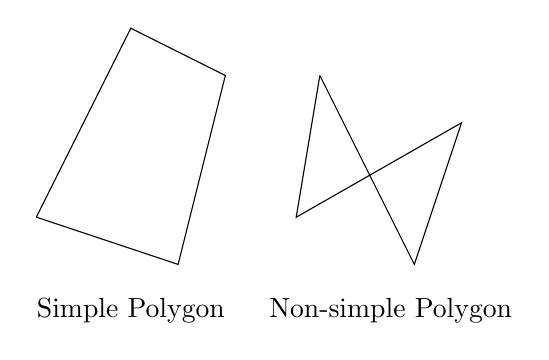
\begin{tikzpicture}[scale=0.6]
					\draw (0, 0) -- (3, -1) -- (4, 3) -- (2, 4) -- (0, 0);
					\draw (6, 3) -- (8, -1) -- (9, 2) -- (5.5, 0) -- (6, 3);
					\node at (2, -1.5) [below] {Simple Polygon};
					\node at (7.5, -1.5) [below] {Non-simple Polygon};
				\end{tikzpicture}
			\end{figure}

			Polygons are basic building blocks in most geometric applications. It can model arbitrarily complex shapes, and apply simple algorithms and algebraic representation/manipulation.
			
		\section{Triangulation}
			\begin{definition}
				\textbf{Triangulation} is to partition polygon $P$ into non-overlapping triangles using diagonals only. It reduces complex shapes to collection of simpler shapes. Every simple $n$-gon admits a triangulation which has $n-2$ triangles.				
			\end{definition}

			\begin{figure}[h!]
				\centering
				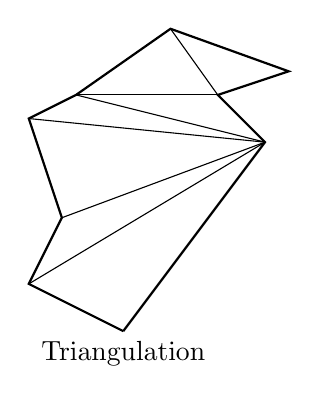
\begin{tikzpicture}[scale=0.6]
					\draw [thick] (0, 0) -- (3, 4) -- (2, 5) -- (3.5, 5.5) -- (1, 6.4) -- (-1, 5) -- (-2, 4.5) -- (-1.3, 2.4) -- (-2, 1) -- (0, 0);
					\draw (-2, 1) -- (3, 4);
					\draw (-1.3, 2.4) -- (3, 4);
					\draw (-2, 4.5) -- (3, 4);
					\draw (-1, 5) -- (3, 4);
					\draw (-1, 5) -- (2, 5);
					\draw (2, 5) -- (1, 6.4);
					\node at (0, 0) [below] {Triangulation};
				\end{tikzpicture}
			\end{figure}

			\begin{theorem}
				Every polygon has a triangulation				
			\end{theorem}
			\begin{lemma}
				Every polygon with more than three vertices has a diagonal.
			\end{lemma}
			\begin{proof}
				(by Meisters, 1975) Let $P$ be a polygon with more than three vertices. Every vertex of a $P$ is either \textit{convex} or \textit{concave}. W.L.O.G.(any polygon must has convex corner) Assume $p$ is a convex vertex. Denote the neighbors of $p$ as $q$ and $r$. If $\bar{qr}$ is a diagonal, done, and we call $\triangle{pqr}$ is an \textit{ear}. If $\triangle{pqr}$ is not an ear, it means at least one vertex is inside $\triangle{pqr}$, assume among those vertexes inside $\triangle{pqr}$, $s$ is a vertex closest to $p$, then $\bar{ps}$ is a diagonal.
			\end{proof}
			
		\section{Art Gallery Theorem}
			\begin{problem}
				The floor plan of an art gallery modeled as a simple polygon with $n$ vertices, there are guards which is stationed at fixed positions with 360 degree vision but cannot see through the walls. How many guards does the art gallery need for the security? (Fun fact: This problem was posted to Vasek Chvatal by Victor Klee in 1973).				
			\end{problem}
			\begin{theorem}
				Every $n$-gon can be guarded with $\lfloor \frac{n}{3} \rfloor$ vertex guards
			\end{theorem}
			\begin{lemma}
				Triangulation graph can be 3-colored.
			\end{lemma}
			\begin{proof}
				- $P$ plus triangulation is a planar graph\\
				- 3-coloring means there exist a 3-partition for vertices that no edge or diagonal has both endpoints within the same set of vertices.\\
				- Proof by Induction:\\
				\indent - Remove an ear (there will always exist ear) \\
				\indent - Inductively 3-color the rest\\
				\indent - Put ear back, coloring new vertex with the label not used by the boundary diagonal.
			\end{proof}

		\section{Triangulation Algorithms}

		\section{Shortest Path}


